\def\firstpage{1}  
\def\lastpage{n}  
\def\lmdcorresp{corr.author@mif.vu.lt}
\def\firstfootnote{0}  
\def\nr{2025}  
% lmd style needs information bellow ======================================  
\def\lmdauthor{Piotr Kuchta\sep Mateusz Knap\and Jakub Szaredko}%Example:% First Author\sep Second Author \and Third Author
\def\lmdtitle{Heralds of War — Projekt koncepcyjny}%Example:% Title of Article  
\def\lmdtitleLT{Straipsnio pavadinimas}%Example:% Straipsnio pavadinimas  
\def\lmdrunauthor{F. Author, S. Author, Th. Author}%Example:% F. Author, S. Author , Th. Author  
\def\lmdruntitle{Runtitle of Article}%Example:% Runtitle of Article  
\def\lmdkeywords{KeyW1EN; KeyW2EN; KeyW3EN;}  
\def\lmdkeywordsLT{KeyW1LT; KeyW2LT; KeyW3LT;}  
\def\lmdams{01AMS01; 01AMS02; 01AMS03}  
   
\def\lmdabstractLT{Abstracto tekstas LT.}  
   
\def\lmdabstract{Abstract text.}  
   
% ************* Author's  references  ******************%  

% ************* end Author's references ******************%  
\documentclass[oneside]{lmdEN}%lmd,lmdRU  
%\input{lmd.def.tex}  
 \makeatletter  

 \spnewtheorem*{west}{Test the West}{\bfseries}{\itshape}  
 \@ifundefined{BibTeX}{%  
 \def\BibTeX{\mbox{{\sc Bib}\TeX}}}{}  
 \makeatother  
% ************* Author's  definitions  ******************%************ Author's  definitions  ******************%  
   
% ************* end Author's definitions ******************%  
\begin{document}  
\bibliographystyle{lmd}  
%  
\begin{topmatter}  
%  \sep  \and Trečias Autorius
%\thankstext{t1}{Title thanks}  
%add runauthor at beginning of Your file  
%add runtitle at beginning of Your file  
%add title at beginning of Your file  
%add add all authors at beginning of Your file  
 \title{\lmdtitle}%Example:% \mmatitle\thanks{Padėka}  
 \author{Piotr Kuchta\sep Mateusz Knap\and Jakub Szaredko}%Example:% First Author${}^{a}\COR{\mmacorresp}\ID{0000-0000-0000-0000}$ \sep Second Author${}^{b}$ \and Last Author${}^{b}$ 
\end{topmatter} 

%  
% ************* Text entry area ******************%  

\section{Tryby gry}

W grze powinny się znaleźć 2-4 tryby gry zdefiniowane poniżej \textit{(jeden też będzie w porządku)}.
\begin{enumerate}
    \item \textbf{Tryb hotseat dla 2 osób} \\
          Do wyboru kilka map zaprojektowanych uprzednio przez
          programistę lub wygenerowanych proceduralnie. Gracze
          wybierają pewien zbiór map oraz jednostek, mogą włączyć ograniczenie na liczbę jednostek danego typu lub całkowicie wyeliminować jednostkę danego typu lub całą klasę. Następnie ustawiają je na pewnym ograniczonym fragmencie planszy.
    \item \textbf{Rozgrywka dla pojedynczego gracza, który walczy z SI} \\
          Mapy zaprojektowane przez programistę lub wygenerowane proceduralnie ułożone są są w pewny ciąg, gdzie jednostki są już określone. Alternatywny wariant pozwalałby na dobór jednostek użytkownikowi na wszystkich lub na pewnej części map, gracz mógłby zobaczyć podgląd mapy przed rozpoczęciem rozgrywki, położenie jednostek byłoby przydzielane ręcznie przez gracza lub pseudo-losowo, być może z algorytmem uwzględniającym klasę jednostki oraz jej statystyk.
    \item \textbf{Rougelike} \\
          Analogicznie jak w punkcie powyższym. Gracz po każdej wygranej bitwie zdobywałby walutę służącą do kupowania jednostek oraz ich ulepszania. Można w tym trybie dodać drzewko technologii, dzięki któremu odblokowywuje się dostęp do kolejnych typów jednostek. Po porażce gra jest zakańczana niepowodzeniem.
    \item \textbf{Komunikacja sieciowa} \\
          Analogicznie jak w punkcie pierwszym. Jeden gracz działa jako host, do którego podłącza się inny gracz.
\end{enumerate}

\section{Opis mechanik gry}

\subsection{Mapa}

Mapa składa się z kwadratowych pól, nie musi posiadać regularnych kształtów, może być np. ścięta z jednej strony, w środku mapy mogą znajdować się też pola wycięte z mapy. Opcjonalnie może występować mgła wojny, która jest rozpraszana za pomocą jednostek, które mają różny zasięg widoczności. Na mapie mogą występować następujące obiekty:

\begin{enumerate}
    \item elementy czysto kosmetyczne, np. krzak, źdźbło trawy;
    \item elementy blokujące, np. drzewo, palisada, jednostki nie mogą na na takie pole wejść, elementy blokujące mogą blokować ataki niektórych jednostek dystansowych;
dystansowych.
    \item \textit{(opcjonalne)} elementy ze skomplikowaną mechaniką:
          \begin{enumerate}
              \item rzeka – zwiększa koszt poruszania się, jeśli jednostka musi przez nią przejść, kary do ataku gdy na niej stoimy;
              \item wzgórze – wzmacnia statystyki ofensywne i defensywne jednostki;
              \item wieża, mur – analogicznie jak w punkcie wyżej;
              \item wilczy dół – zadaje obrażenia jednostkom, które na niego wejdą.
          \end{enumerate}
\end{enumerate}

\subsection{System walki}

Tury graczy następują w pętli po sobie. Tura składa się z pojedynczych sekwencji przypisanych do graczy, ich liczba jest zdefiniowana za pośrednictwem liczby żyjących jednostek w aktualnej turze, ich kolejność będzie zdefiniowana za pomocą prostego algorytmu, np. \textit{ABAABB…}, gdzie \textit{A} i \textit{B} to gracze lub bardziej zaawansowanego algorytmu, który będzie zależny od wyniku poprzedniej tury lub tur. Odblokowanie jednej sekwencji pozwoli na wykonanie akcji dowolną jednostką gracza w obrębie jej staminy. Akcja to ruch, atak, wykorzystanie umiejętności wykonane zero (bezczynność) lub więcej razy. \\\\\noindent
Stamina to bardzo ważny zasób określający możliwości danej jednostki, wykorzystywany do wykonania akcji. Każda jednostka ma swój indywidualny poziom staminy. Ilość staminy można regulować poprzez, np. ulepszenia w trybie roguelike. Po wykonaniu akcji w danej sekwencji stamina zostaje częściowo lub całkowicie odnowiona, natomiast po zakończeniu tury stamina pozostaje odnowiona wszystkim jednostkom. \\\\\noindent
Jednostki mogą być zwrócone w czterech kierunkach, kierunek jest zdeterminowany przez ostatni ruch jednostki w kwadracie lub za pomocą algorytmu, który przeanalizuje położenie wrogich jednostek i podejmie decyzje o najlepszej rotacji. Jednostki posiadają dwie strefy w walce defensywnej: neutralną i wrażliwą, zależne od pozycji atakującej jednostki przeciwnika i kierunku jednostki atakowanej. Strefa wrażliwa zmniejsza statystyki defensywne, a neutralna, jak nazwa wskazuje, pozostawia je bez zmian. Strefy i ich zależność od rotacji jednostek zostały przedstawione na \hyperref[fig:unit-rotation]{\underline{schemacie}}.\\\\\noindent
Jednostki długodystansowe mogą atakować w dowolnym kierunku. Jeśli trajektoria pocisku przechodzi przez pole z elementem blokującym, obrażenia są skalowane w dół. Wartość obrażeń przemnażana jest przez stosunek wyciętego przez trajektorię trójkąta prostokątnego lub trapezu danego kwadratu do całkowitego pola powierzchni kwadratu, jeśli pole powierzchni wyciętej figury jest równe $50\%$ pola powierzchni kwadratu, to wtedy obrażenia są zerowe \textit{(trafiamy bezpośrednio w przeszkodę)}.

\begin{figure}[ht]
\centering
\begin{minipage}{.5\textwidth}
  \centering
  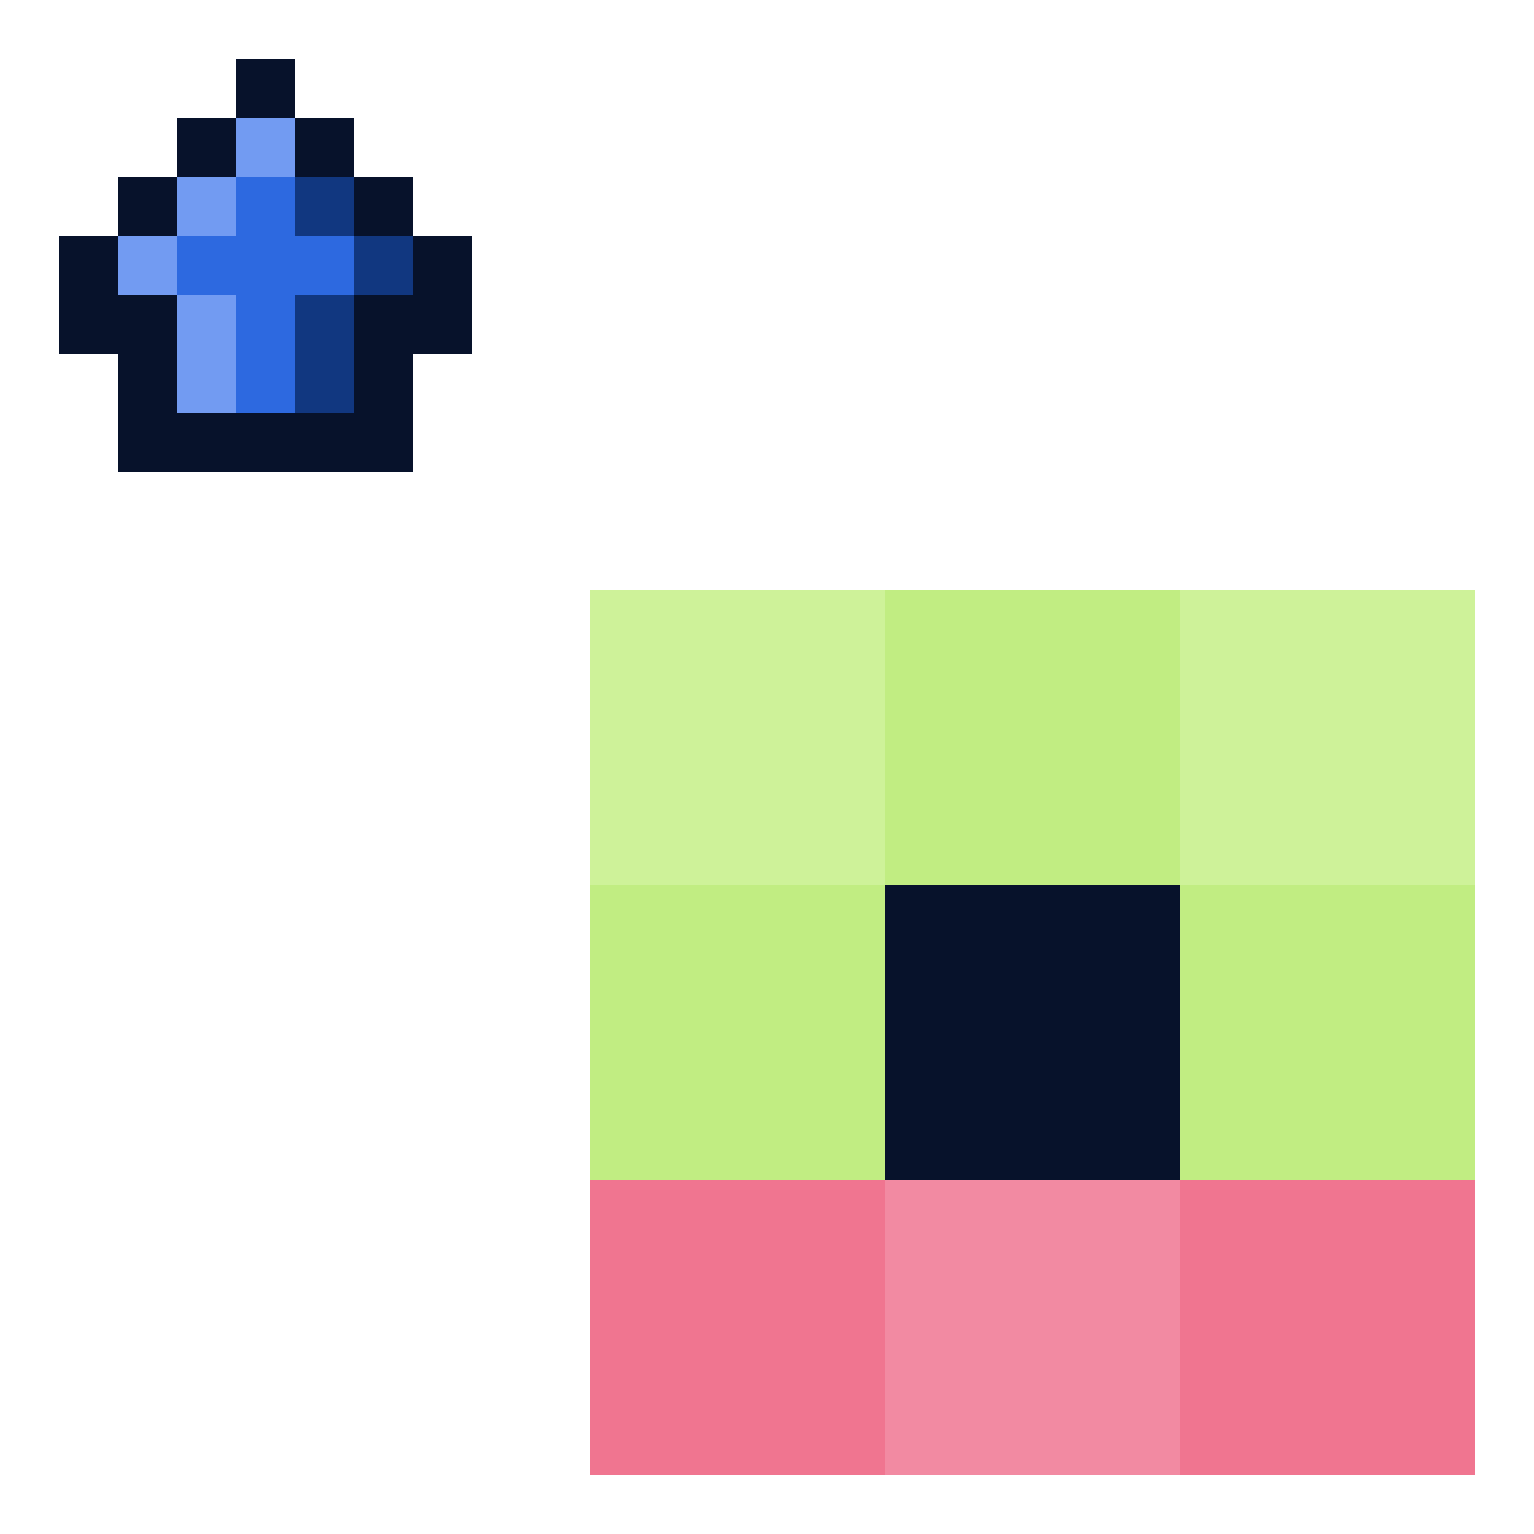
\includegraphics[width=.8\linewidth]{images/unit-rotation-n.png}
  \captionof{figure}{Jednostka skierowana w górę}
  \label{fig:unit-rotation-n}
\end{minipage}%
\begin{minipage}{.5\textwidth}
  \centering
  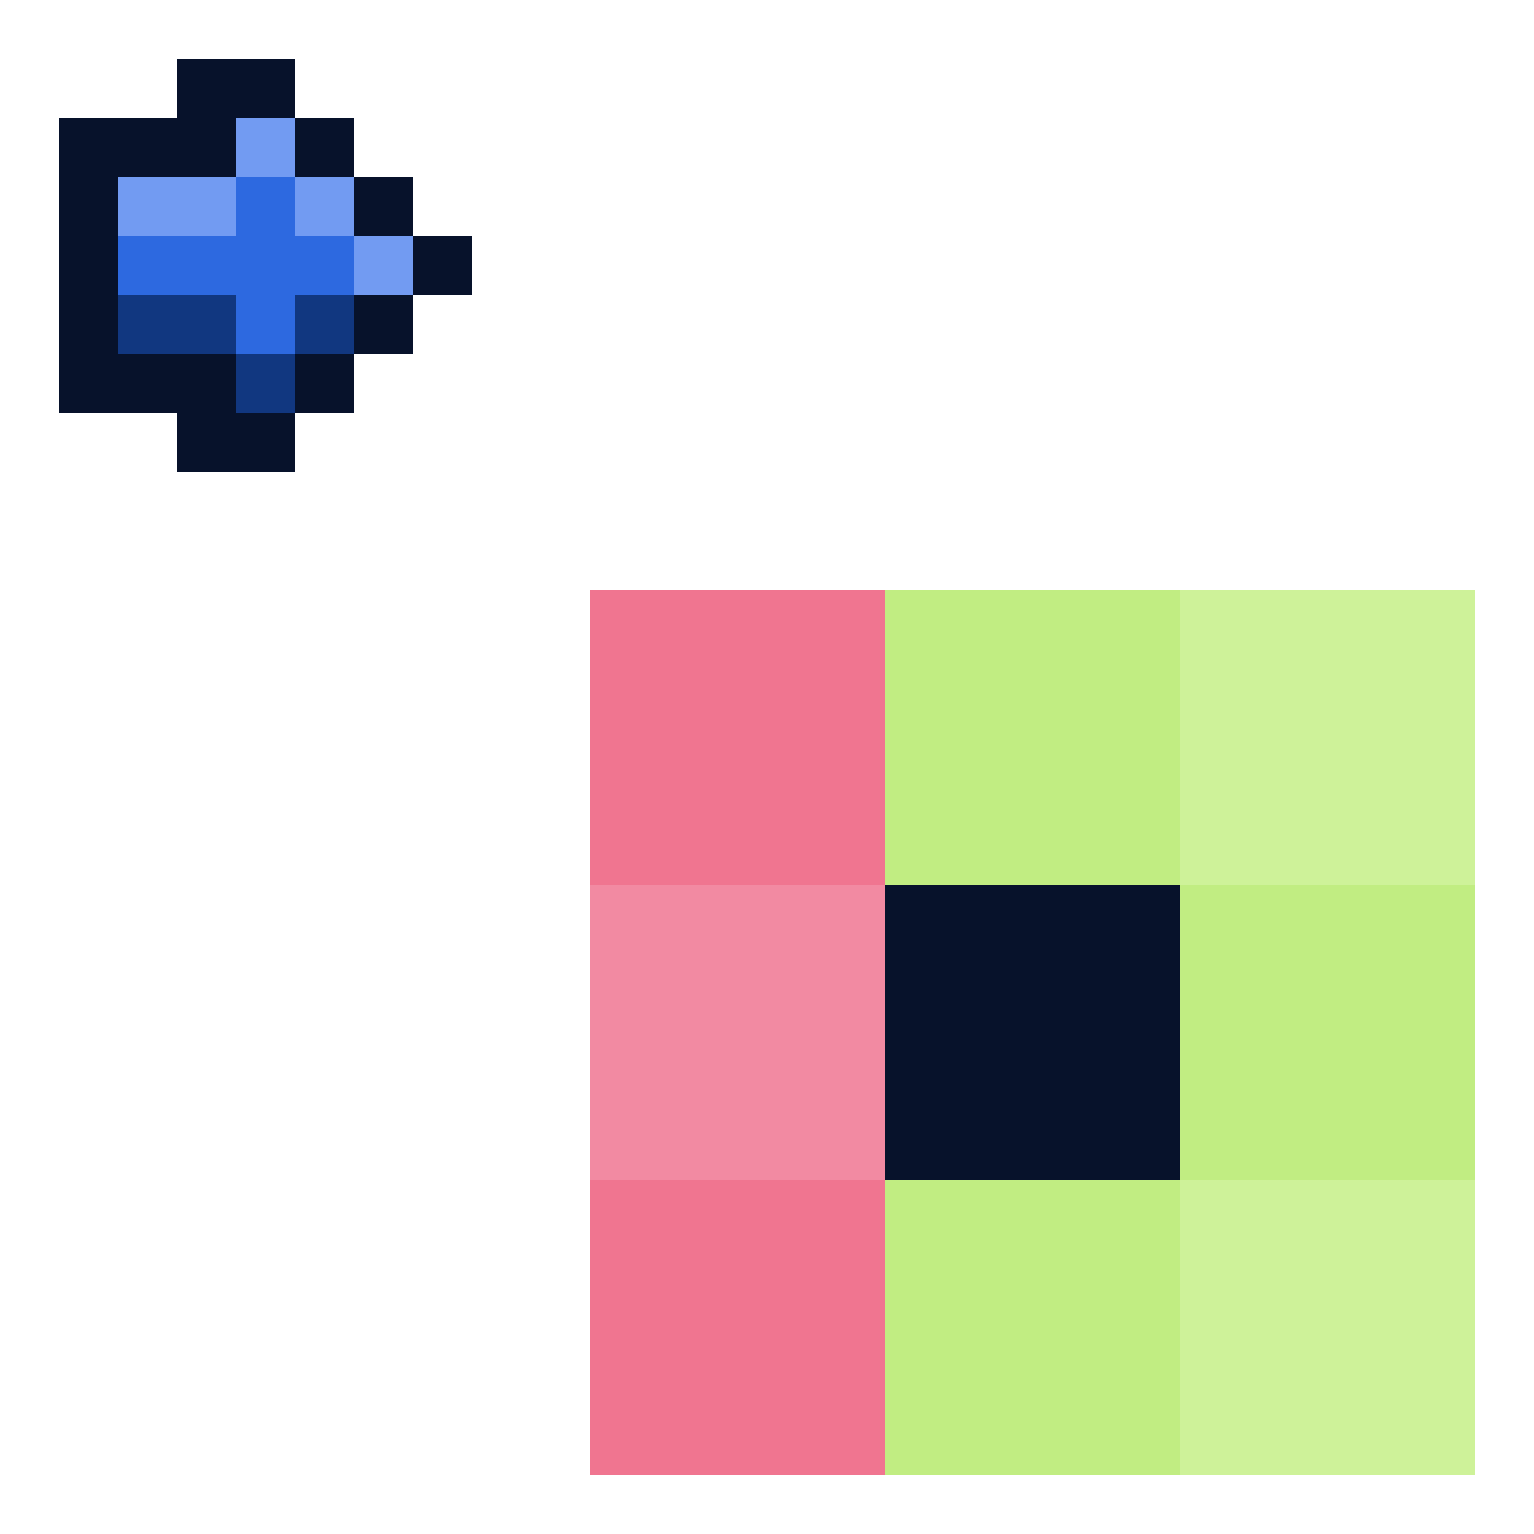
\includegraphics[width=.8\linewidth]{images/unit-rotation-e.png}
  \captionof{figure}{Jednostka skierowana w prawo}
  \label{fig:unit-rotation-e}
\end{minipage}
\vskip 1em
\begin{minipage}{.5\textwidth}
  \centering
  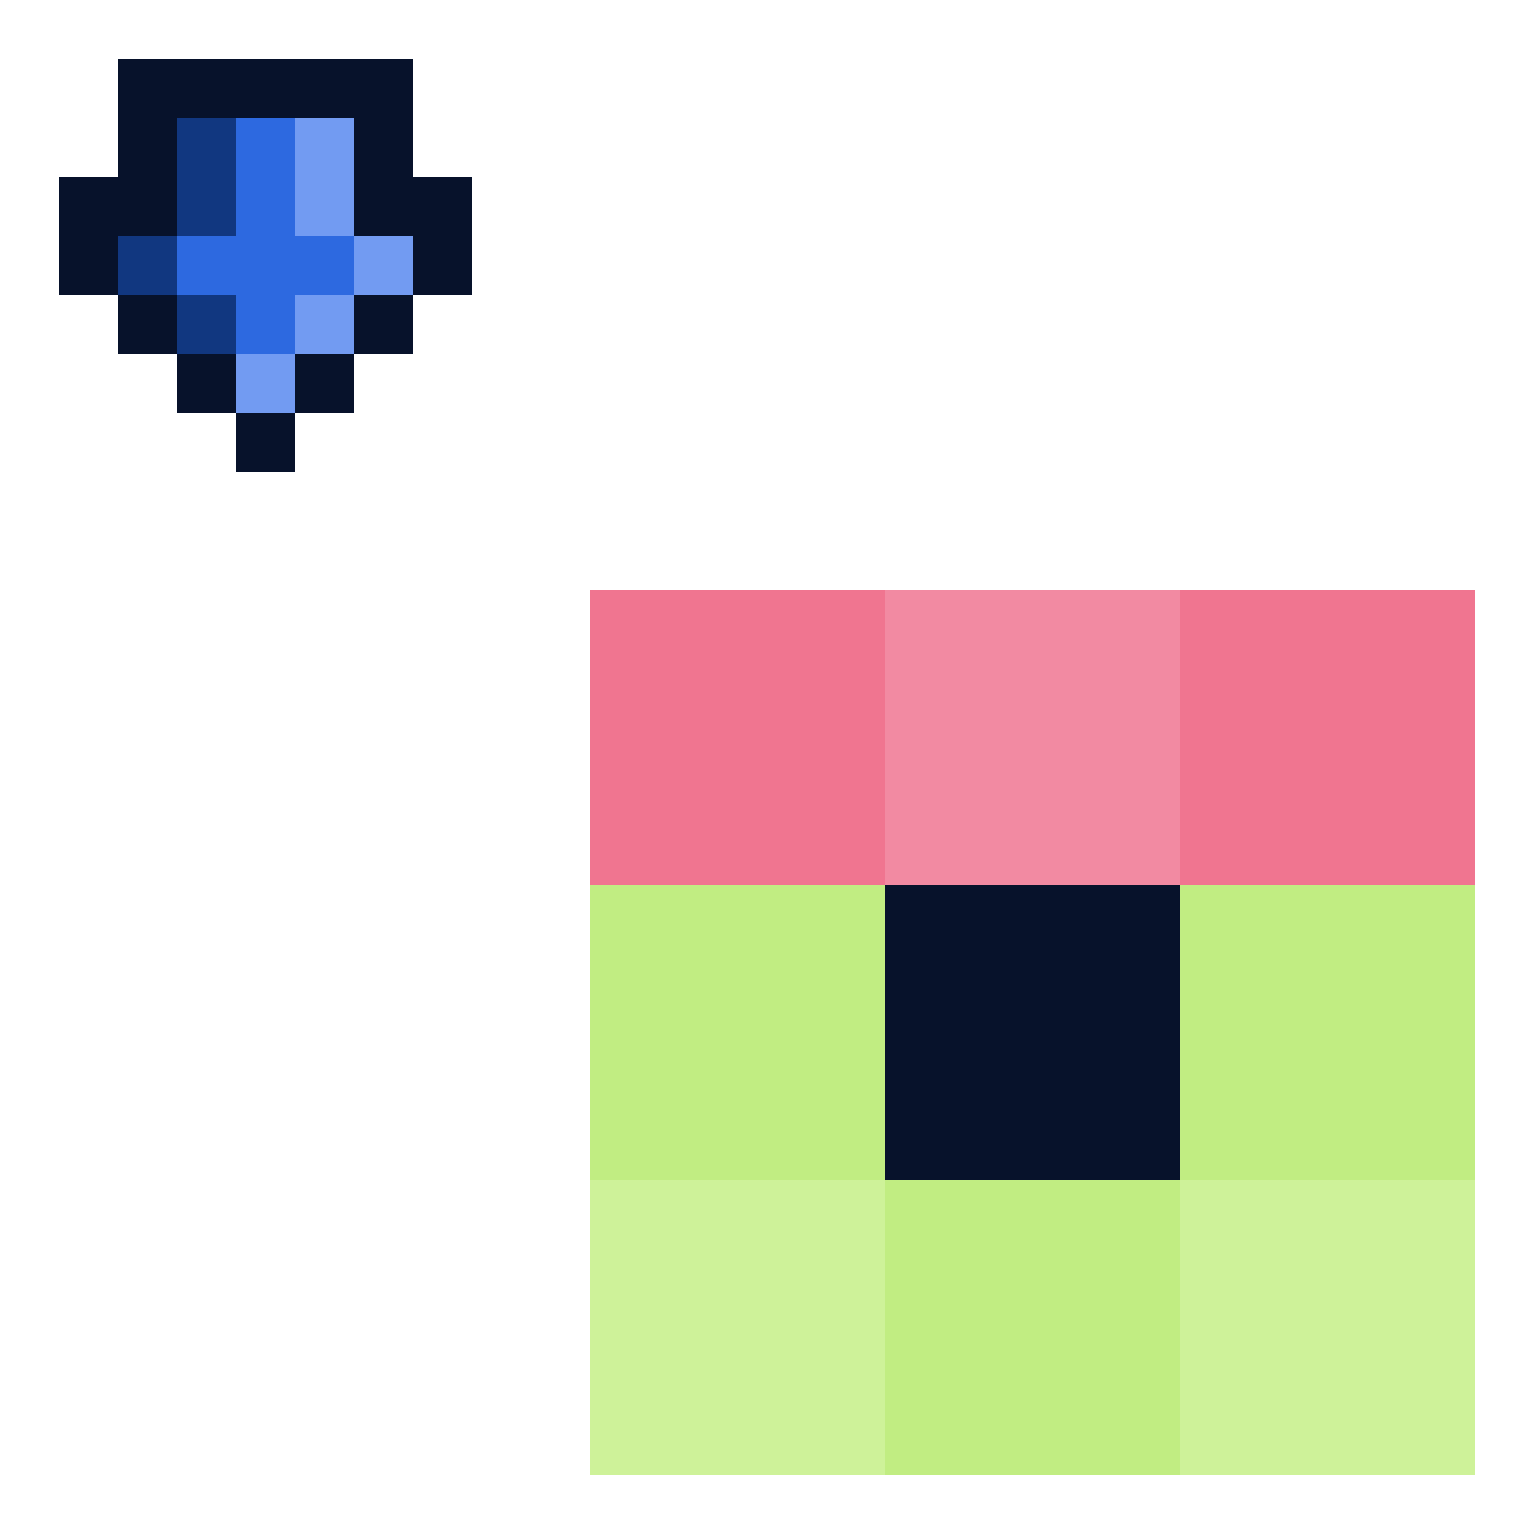
\includegraphics[width=.8\linewidth]{images/unit-rotation-s.png}
  \captionof{figure}{Jednostka skierowana w dół}
  \label{fig:unit-rotation-s}
\end{minipage}%
\begin{minipage}{.5\textwidth}
  \centering
  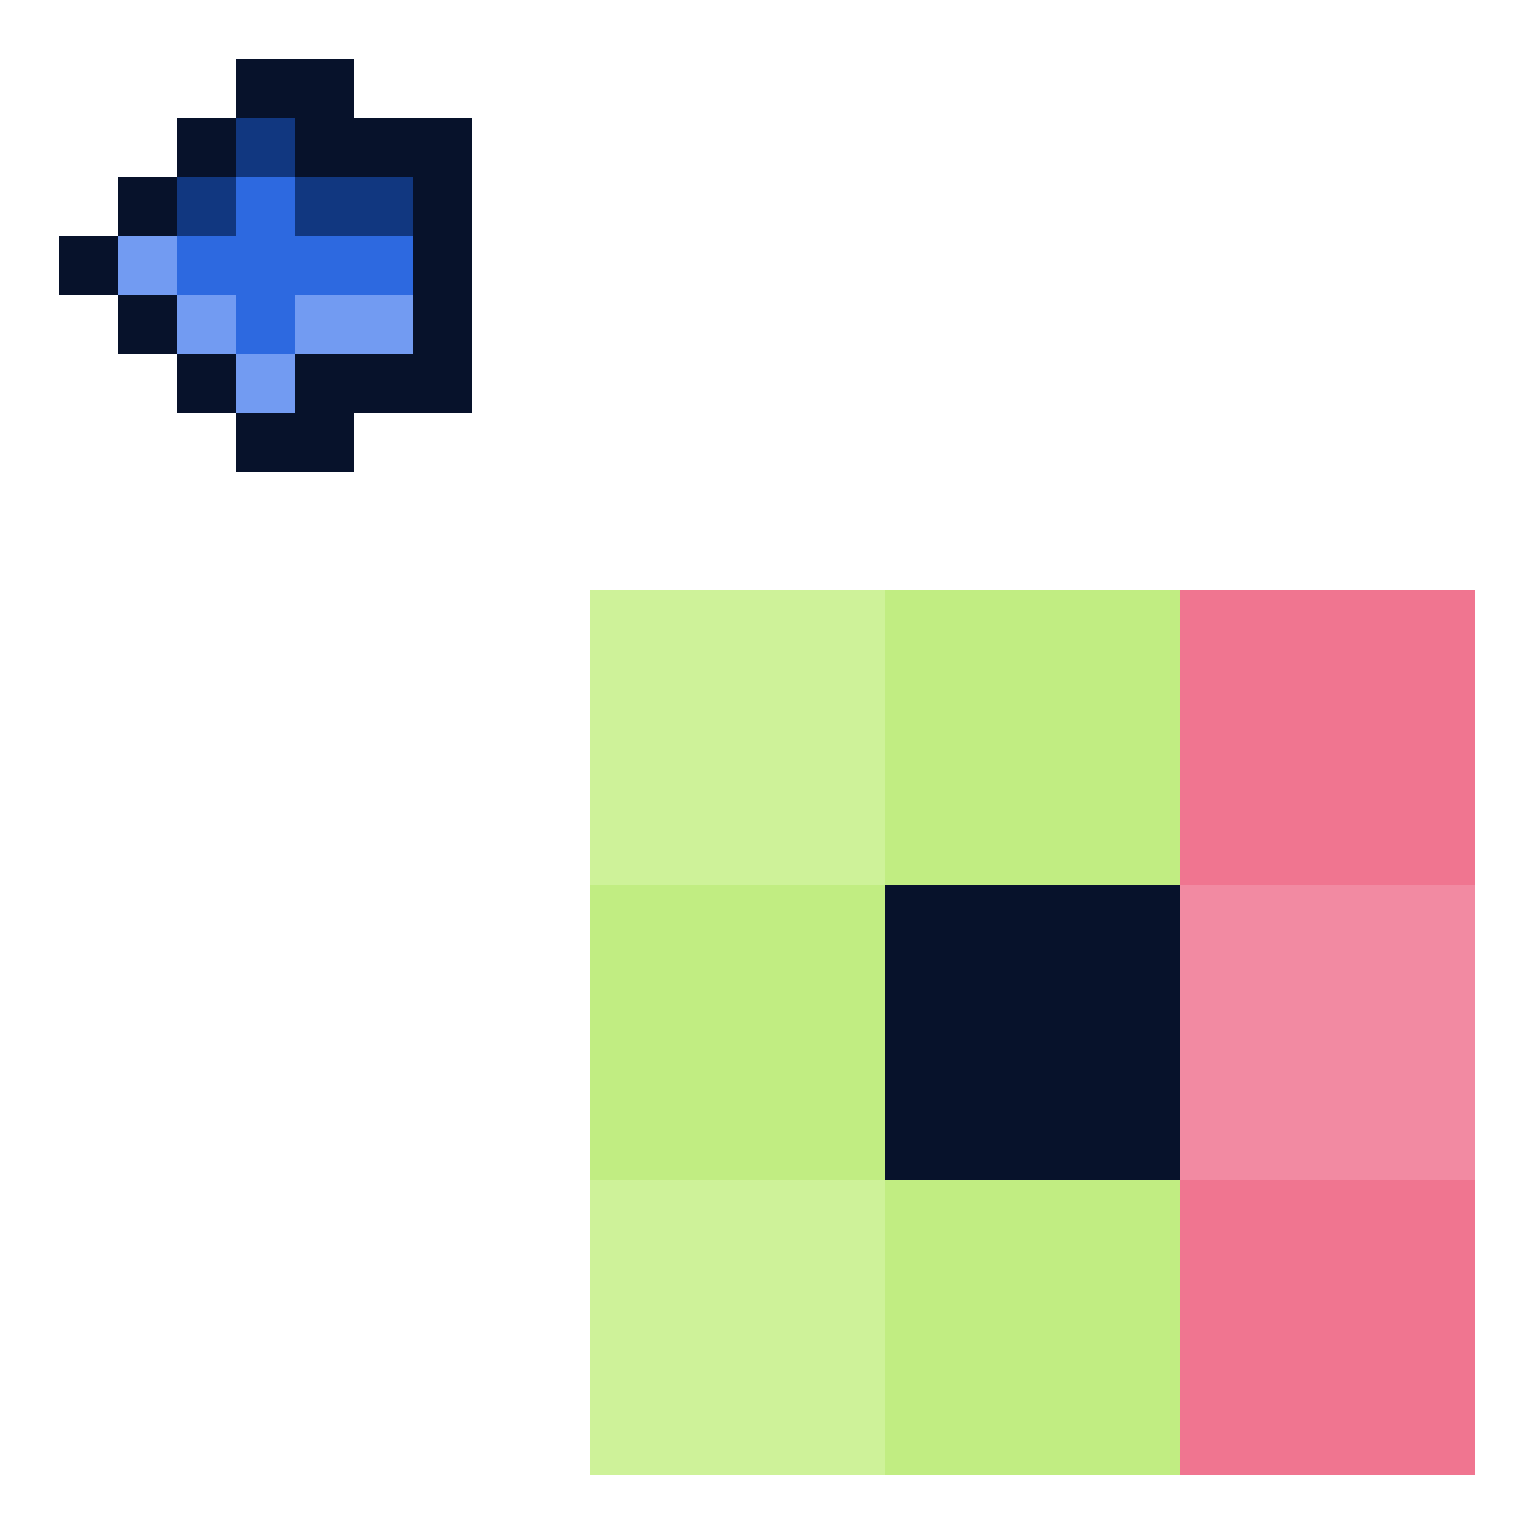
\includegraphics[width=.8\linewidth]{images/unit-rotation-w.png}
  \captionof{figure}{Jednostka skierowana w lewo}
  \label{fig:unit-rotation-w}
\end{minipage}
\label{fig:unit-rotation}
\end{figure}

\section{Jednostki}

Jednostki mogą się poruszać we wszystkich kierunkach, zmieniają swój obrót w zależności od kierunku ruchu w dwóch sąsiednich polach. Ich zasięg poruszania się to koło \textit{(w przybliżeniu, ponieważ ograniczenie planszy do relatywnie małej siatki nie umożliwi na reprezentację koła w pełni)}. Zasięg jednostki jest zależny od poziomu staminy, różne jednostki mogą mieć różną jej ilość, elementy występujące na mapie wpływają na staminę.\\\\\noindent

\subsection{Podstawowe klasy}
Wyodrębniamy trzy podstawowe klasy jednostek:
\begin{enumerate}
    \item \textbf{Walczące w zwarciu}\\
          Muszą podejść bezpośrednio do atakowanej jednostki, zasięg ataku jest równy jedną lub dwie kratki. Zazwyczaj posiadają dobre statystyki defensywne.
    \item \textbf{Zasięgowe}\\
          Posiadają znaczący zasięg ataku w kształcie koła o promieniu większym niż dwie kratki. Strategia ich walki polega na utrzymywaniu ciągłego dystansu z wrogimi jednostkami, \textit{choć to nie wyklucza możliwości walki wręcz}. Zazwyczaj posiadają słabe statystyki defensywne, natomiast dobre statystyki ofensywne.
    \item \textbf{Specjalne}\\
          Nie należą do dwóch powyższych klas aczkolwiek mogą walczyć zarówno w zwarciu jak i na dystans. Są to jednostki do specjalnych zadań, którym głównym zadaniem nie jest zadawanie obrażeń. Do tej klasy należą między innymi inżynierowie.
\end{enumerate}

\subsection{Typy}

\begin{enumerate}
    \item Walczące w zwarciu
          \begin{enumerate}
              \item \textbf{Piechota}
                    \begin{itemize}
                        \item Ofensywa: $\blacksquare\blacksquare\blacksquare\blacksquare\square\square\square\square$
                        \item Defensywa: $\blacksquare\blacksquare\blacksquare\blacksquare\blacksquare\blacksquare\square\square$
                        \item Zasięg ataku: 1 pole
                        \item Stamina: $\blacksquare\blacksquare\blacksquare\square\square\square\square\square$
                    \end{itemize}
              \item \textbf{Pikinierzy}
                    \begin{itemize}
                        \item Ofensywa: $\blacksquare\blacksquare\blacksquare\square\square\square\square\square$
                        \item Defensywa: $\blacksquare\blacksquare\blacksquare\blacksquare\square\square\square\square$
                        \item Zasięg ataku: 2 pola
                        \item Stamina: $\blacksquare\blacksquare\blacksquare\square\square\square\square\square$
                        \item Bonus do walki z konnicą
                    \end{itemize}
              \item \textbf{Kawaleria}
                    \begin{itemize}
                        \item Ofensywa: $\blacksquare\blacksquare\blacksquare\blacksquare\square\square\square\square$, obrażenia skalujące się od liczby przebytych pól w sekwencji
                        \item Defensywa: $\blacksquare\blacksquare\blacksquare\square\square\square\square\square$
                        \item Zasięg ataku: 1 pole
                        \item Stamina: $\blacksquare\blacksquare\blacksquare\blacksquare\blacksquare\blacksquare\square\square$
                        \item Kara do walki z pikinierami
                    \end{itemize}
              \item \textbf{Tarczownicy}
                    \begin{itemize}
                        \item Ofensywa: $\blacksquare\square\square\square\square\square\square\square$
                        \item Defensywa: $\blacksquare\blacksquare\blacksquare\blacksquare\blacksquare\blacksquare\blacksquare\blacksquare$
                        \item Zasięg ataku: 1 pole
                        \item Stamina: $\blacksquare\blacksquare\square\square\square\square\square\square$
                        \item Zadawanie obrażeń atakującym jednostkom
                    \end{itemize}
          \end{enumerate}
    \item Zasięgowe
          \begin{enumerate}
              \item \textbf{Łucznicy}
                    \begin{itemize}
                        \item Ofensywa: $\blacksquare\blacksquare\blacksquare\blacksquare\blacksquare\square\square\square$
                        \item Defensywa: $\blacksquare\square\square\square\square\square\square$
                        \item Zasięg ataku: 8 pól
                        \item Stamina: $\blacksquare\blacksquare\blacksquare\blacksquare\square\square\square\square$
                    \end{itemize}
              \item \textbf{Kusznicy}
                    \begin{itemize}
                        \item Ofensywa: $\blacksquare\blacksquare\blacksquare\blacksquare\blacksquare\blacksquare\square\square$
                        \item Defensywa: $\blacksquare\blacksquare\blacksquare\square\square\square\square$
                        \item Zasięg ataku: 6 pól
                        \item Stamina: $\blacksquare\blacksquare\blacksquare\square\square\square\square\square$
                    \end{itemize}
              \item \textbf{Arkebuzerzy}
                     \begin{itemize}
                        \item Ofensywa: $\blacksquare\blacksquare\blacksquare\blacksquare\blacksquare\blacksquare\blacksquare\square$
                        \item Defensywa: $\blacksquare\blacksquare\square\square\square\square\square$
                        \item Zasięg ataku: 4 pola
                        \item Stamina: $\blacksquare\blacksquare\blacksquare\square\square\square\square\square$
                    \end{itemize}
              \item \textbf{Łucznicy na koniach}
                    \begin{itemize}
                        \item Ofensywa: $\blacksquare\blacksquare\blacksquare\blacksquare\square\square\square\square$
                        \item Defensywa: $\blacksquare\square\square\square\square\square\square$
                        \item Zasięg ataku: 5 pól
                        \item Stamina: $\blacksquare\blacksquare\blacksquare\blacksquare\blacksquare\blacksquare\blacksquare\square$
                    \end{itemize}
              \item \textbf{Armaty}
                    \begin{itemize}
                        \item Ofensywa: $\blacksquare\blacksquare\blacksquare\blacksquare\blacksquare\blacksquare\blacksquare\blacksquare$
                        \item Defensywa: $\square\square\square\square\square\square\square$
                        \item Zasięg ataku: 9 pól
                        \item Stamina: $\square\square\square\square\square\square\square$
                    \end{itemize}
          \end{enumerate}
    \item Specjalne
          \begin{enumerate}
              \item \textbf{Inżynierowie}
                    \begin{itemize}
                        \item Ofensywa: $\square\square\square\square\square\square\square$
                        \item Defensywa: $\square\square\square\square\square\square\square\square$
                        \item Zasięg ataku: 1 pole
                        \item Stamina: $\blacksquare\blacksquare\blacksquare\square\square\square\square\square$
                        \item Umiejętności
                              \begin{itemize}
                                  \item Budowanie wilczych dołów, palisad, wież; zużywa bardzo dużo punktów staminy
                                  \item Naprawianie pewnych jednostek, np. armat.
                                  \item Ulepszanie jednostek
                              \end{itemize}
                    \end{itemize}
          \end{enumerate}

    
\end{enumerate}

%spell_to this point %********** End of text entry *****************%  
%\begin{thebibliography}{9}  
%\end{thebibliography}  

% ---------------------------------------  

\end{document}  
   
   

